\documentclass[letterpaper,11pt]{article}

\usepackage{listings}
\usepackage{color}

\definecolor{dkgreen}{rgb}{0,0.6,0}
\definecolor{gray}{rgb}{0.5,0.5,0.5}
\definecolor{mauve}{rgb}{0.58,0,0.82}

\lstset{frame=tb,
  language=Python,
  aboveskip=3mm,
  belowskip=3mm,
  showstringspaces=false,
  columns=flexible,
  basicstyle={\small\ttfamily},
  numbers=none,
  numberstyle=\tiny\color{gray},
  keywordstyle=\color{blue},
  commentstyle=\color{dkgreen},
  stringstyle=\color{mauve},
  breaklines=true,
  breakatwhitespace=true,
  tabsize=3
}

\usepackage{setspace}
\usepackage{graphicx}
\usepackage{bm}    %for textbf
\usepackage{amsmath}
\usepackage{amsfonts}   %for mathbb
\allowdisplaybreaks[4]  %from {amsmath}
\newcommand{\independent}{\rotatebox[origin=c]{90}{$\models$}}  %from {graphicx}
\usepackage{geometry}
\geometry{letterpaper, scale=0.8}  %from {geometry}
\author{Yuan Yin}
\title{EECS 545 Homework 3}
\begin{document}\large
\maketitle
\begin{spacing}{1.2}  %from {setspace}
\section*{Problem 2}
\subsection*{(b) \& (c)}
Code and result is as follows:
\begin{lstlisting}
import numpy as np
import matplotlib.pyplot as plt
import pylab as pl

n = 200
np.random.seed(0) # Seed the random number generator
x = np.random.rand(n,1)
z = np.zeros([n,1])
k = n * 0.4
rp = np.random.permutation(n)
outlier_subset = rp[1:int(k)]
z[outlier_subset] = 1 # outliers
y = (1 - z) * (10 * x + 5 + np.random.randn(n,1)) + z * (20 - 20 * x + 10 * np.random.randn(n,1))

# Plot data and true line
plt.scatter(x, y, label = 'data')

t = pl.frange(0,1,0.01)
plt.plot(t, 10*t+5, 'k-', label = 'true line')

# Add your code for ordinary least squares below
x_ols = np.mat(x); y_ols = np.mat(y) # They are all 200*1 matrix
y_mdf = y_ols - np.mean(y_ols); x_mdf = x_ols - np.mean(x_ols)
A = 2 * (x_mdf.T * x_mdf); r = -2 * x_mdf.T * y_mdf; c = y_mdf.T * y_mdf
w_ols = -(A.I * r)[0,0]; b_ols = np.mean(y_ols) - w_ols * np.mean(x_ols)
print("Parameters of OLS are: w: ",w_ols, "b: ", b_ols)

plt.plot(t, w_ols*t+b_ols, 'g--', label = 'least squares')

#######################################################
# helper function to solve weighted least squares
    # add your code here
def wls(x,y,c):
    add = 1
    x_add = np.insert(x, 0, values=add, axis=1)
    theta = (x_add.T * c * x_add).I * x_add.T * c * y
    b = theta[0]; w = theta[1]
    return w, b

# Add your code for robust regression MM algorithm below
x_rob = np.mat(x); y_rob = np.mat(y)
w_rob = 0; b_rob = 0
error = 1
while error > 0.01:
    c = np.eye(len(x_rob))
    for i in range(len(x_rob)):
        r_t_i = y_rob[i] - w_rob * x_rob[i] - b_rob
        c[i,i] = 1/(2*np.sqrt(1+r_t_i**2))
    w_new, b_new = wls(x_rob, y_rob, c)
    error = np.sqrt((w_new - w_rob)**2 + (b_new - b_rob)**2)
    w_rob, b_rob = w_new[0,0], b_new[0,0]

print("Parameters of ROB are: w: ",w_rob, "b: ", b_rob)
plt.plot(t, w_rob*t+b_rob, 'r:', label = 'robust')
legend = plt.legend(loc='upper right', shadow=True)
plt.show()
\end{lstlisting}
the result is:
\begin{lstlisting}
Parameters of OLS are: w: -1.4749427077811519 b: 10.519708850514508
Parameters of robust regression are: w: 7.302235544182917 b: 6.186315755157274
\end{lstlisting}
the plot which shows the data, the true line, the OLS estimate and the robust estimate is as bellow:

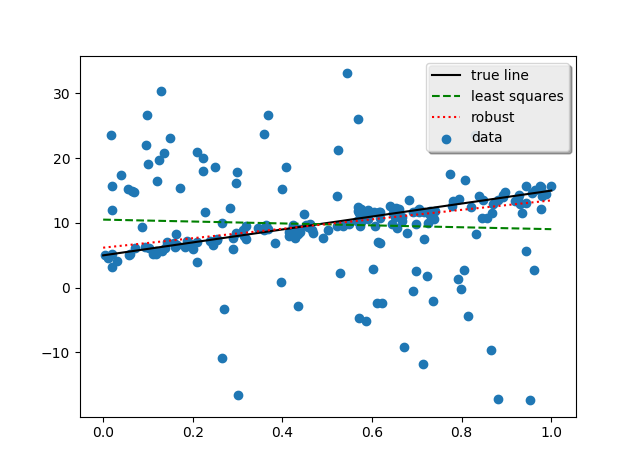
\includegraphics[width=4.95in,height=4.05in]{Robust_Regression.png}

\section*{Problem 4}

the code and the result is as follows:
\begin{lstlisting}
from numpy import *
import numpy as np
import scipy.io as sio
import matplotlib.pyplot as plt

# Import the data
mnist_49_3000 = sio.loadmat('mnist_49_3000.mat')
x = mnist_49_3000['x']
y = mnist_49_3000['y']
d,n = x.shape
y += (y < 0) * 1

# Process the data, we divide the data into training part and test part
added = np.ones(n)
x_original = x; y_original = y
x = mat(np.vstack((added,x))); y = mat(y)
x_train = x[:,:2000]; y_train = y[:,:2000]
x_test = x[:,2000:]; y_test= y[:,2000:]

# Initialize parameters
lamda = 10
theta = mat(np.zeros(d + 1))
dJ = mat(np.zeros(d + 1))
d2J = mat(np.zeros([d + 1,d + 1]))

# Iteration with Newton's Method:
## Notice here the stop condition for iteration is when the change of theta is less than 1%
N = 0; error0 = 10
while (error0 > 0.01):
    z = 1 / (1 + np.exp(-theta*x_train))
    dJ = x_train*(z-y_train).T+2*lamda*theta.T
    d2J = x_train * mat(diag(multiply(z, (1-z)).getA()[0])) * x_train.T + 2*lamda*mat(np.eye(d+1,d+1))
    error0 = np.sqrt(((d2J.I * dJ).T * (d2J.I * dJ))[0,0])
    theta = theta - (d2J.I * dJ).T
    y_train_result = theta * x_train
    for l in range(2000):
        if y_train_result[0,l] < 0:
            y_train_result[0,l] = 0
        else:
            y_train_result[0,l] = 1
    N = N+1
print("Iteration times: ", N)
log_like = 0
for l in range(2000):
    z = 1 / (1 + np.exp(-theta * x_train[:,l]))
    log_like += y_train[0,l]*np.log(z)+(1-y_train[0,l])*np.log(1-z)
J = -log_like + lamda*theta*theta.T
print("Value of objective function is: ", J[0,0])

# Test data
y_test_result = theta * x_test
eta_test = 1/(1+np.exp(-y_test_result))
false = []
for l in range(1000):
    if y_test_result[0, l] < 0:
        y_test_result[0, l] = 0
    else:
        y_test_result[0, l] = 1
error1 = 0
for m in range(1000):
    if y_test_result[0, m] != y_test[0, m]:
        error1 += 1
        false.append(m)
print("Test error is: ", error1/1000)
prob = np.zeros(1000)
x_false = x_test[1:,false]; x_false = x_false.getA()
y_false = y_test[:,false]
y_false_result = y_test_result[:,false]
for l in range(1000):
    if y_test_result[0,l] == 0:
        prob[l] = 1-eta_test[0,l]
    else:
        prob[l] = eta_test[0,l]
confidence = prob[false]
indx = argsort(confidence)[28:]
x_false20 = np.zeros((d,20)); y_real20 = np.zeros(20); y_pre20 = np.zeros(20)
for l in range(20):
    x_false20[:,l] = x_false[:,int(indx[l])]
    y_real20[l] = y_false[:,int(indx[l])]
    y_pre20[l] = y_false_result[:,int(indx[l])]

## Plot the picture of 20 most confident missclassified pictures
fig =  plt.figure(num='missclassified',figsize=(8,8))
fig.suptitle("\"True\" represents real result, \"Pre\" represents predicted result\n")
for l in range(20):
    plt.subplot(4,5,1+l)
    if y_real20[l] == 0:
        true_title = 4
        pre_title = 9
    else:
        true_title = 9
        pre_title = 4
    plt.title('True: %s, Pre: %s' %(str(true_title), str(pre_title)))
    plt.imshow(np.reshape(x_false20[:,l], (int(np.sqrt(d)), int(np.sqrt(d)))))
plt.show()
plt.close()
\end{lstlisting}
the result is:

\begin{lstlisting}
Iteration times:  6
Value of objective function is:  307.65546352880267
Test error is:  0.048
\end{lstlisting}
\end{spacing}
\end{document}